% 2010 年陕西卷理科第 15 题【B】：Rt△ABC 与以 AC 为直径的圆。
% 来源 PDF：普通高考/2010/2010陕西理.pdf，SHA-256 8406e303e7aa1ac7813893781c903a7d9c904530028e6fd1c06062d1c32bd645。
% 原页：第 1 页（A3 三栏）第 3 栏上部，书页码 623。
% 重绘依据：照原页——A 在最高处，C 在其正下方（直角顶点，直角符号朝内），B 在左下方；
%   圆以 AC 为直径（圆心 O 标出圆点），圆周向右鼓出 AC 之外；斜边 AB 与圆交于 D（D 在 A 与 B 之间）。
%   按题设 AC=3、BC=4 取坐标：C=(0,0)，A=(0,3)，B=(-4,0)，则 D=(-1.44,1.92)。
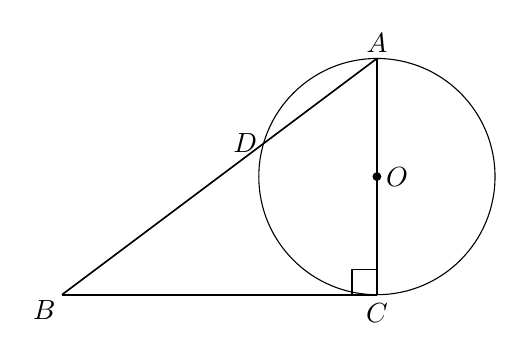
\begin{tikzpicture}[semithick, line join=round]
  \coordinate (C) at (0,0);
  \coordinate (A) at (0,3);
  \coordinate (B) at (-4,0);
  \coordinate (O) at (0,1.5);
  \coordinate (D) at (-1.44,1.92);

  % 以 AC 为直径的圆
  \draw[thin] (O) circle (1.5);

  % 三角形三边
  \draw (A) -- (B);
  \draw (B) -- (C);
  \draw (C) -- (A);

  % C 处直角符号
  \draw (0,0.32) -- (-0.32,0.32) -- (-0.32,0);

  % 圆心
  \fill (O) circle (1.6pt);

  % 顶点与交点标注
  \node[above, inner sep=2pt] at (A) {$A$};
  \node[below left, inner sep=2pt] at (B) {$B$};
  \node[below, inner sep=3pt] at (C) {$C$};
  \node[right, inner sep=3pt] at (O) {$O$};
  \node[left, inner sep=2pt] at (D) {$D$};
\end{tikzpicture}
